\documentclass[a4paper,10pt]{article}

\usepackage[space,fontset=fandol]{ctex}

\usepackage{graphicx}
\usepackage{minted}

\setminted{frame=lines,linenos=true,mathescape=true,escapeinside=||}

\newcommand{\ttvariable}[1]{\texttt{\textit{#1}}}

\title{简单的社交网络程序}
\author{伏贵荣 郭一江 曾浩}
\date{\today}

\begin{document}

\maketitle

\section{简介}

本程序是一个简单的社交网络程序, 实现了一个社交网络的基本功能:
\begin{enumerate}
	\item 用户的注册,登录检查;
	\item 允许用户查询自己的好友,允许用户 post 自己的状态,查看和回复用户的状态;
	\item 用户登录页面主页时,每隔 30 秒钟,如果用户的好友有更新的状态,自动更新最新的用户好友状态.
	\item 支持查看好友的好友信息;
	\item 有多种个性化的头像可供选择.
\end{enumerate}

为了体现对数据库管理系统的应用, 本程序中尽可能使用 SQL 语句完成核心功能.

\section{数据库设计}

\subsection{实体--关系图 (E-R 图)}

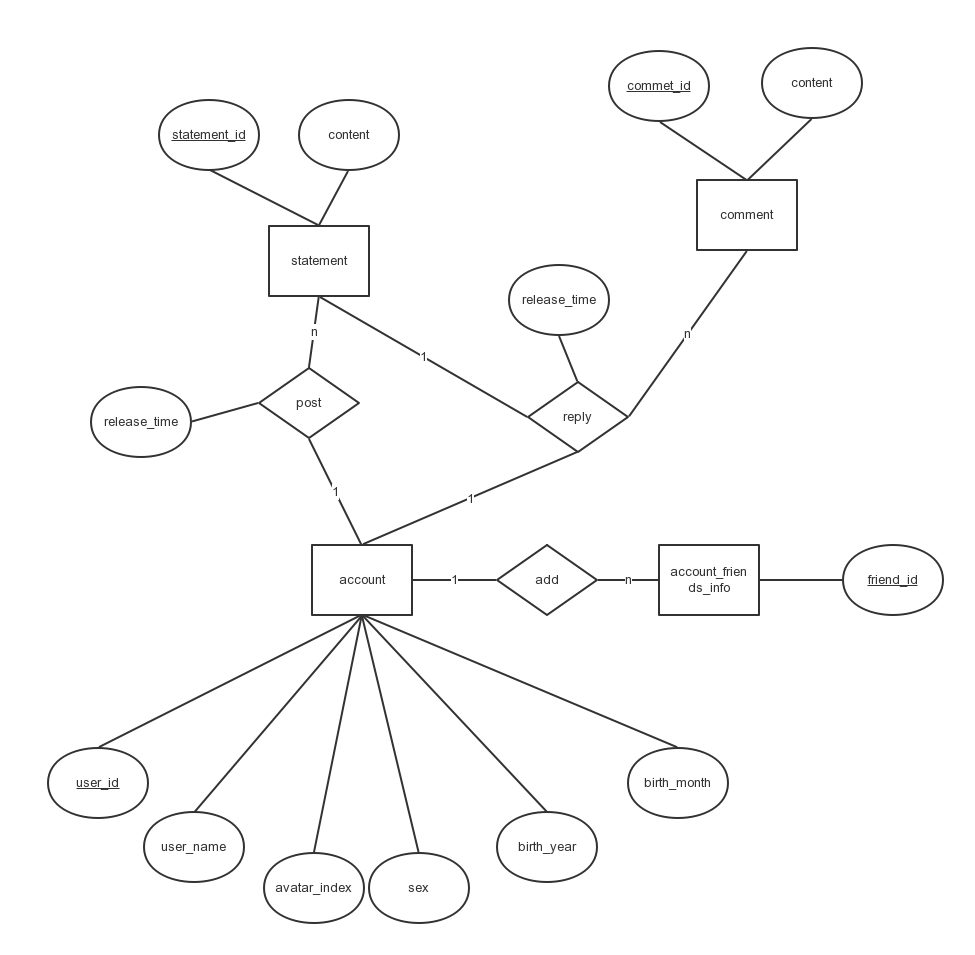
\includegraphics[width=\linewidth]{erd.png}

\subsection{数据库表结构}

数据库分为 4 个表:
\begin{itemize}
	\item \mintinline{text}{account}, 用户账户表;
	\item \mintinline{text}{friends}, 好友列表;
	\item \mintinline{text}{statement}, 用户发表的状态;
	\item \mintinline{text}{comment}, 用户对好友状态的评论.
\end{itemize}

\mintinline{text}{account} 表记录用户的基本信息.
\begin{center}
	\begin{tabular}{ccc} \hline 
		列名 & 类型 & 属性 \\ \hline
		\mintinline{text}{user_id} & char(16) & 主键 \\
		\mintinline{text}{password} & char(32) & \\
		\mintinline{text}{user_name} & char(16) & \\
		\mintinline{text}{avatar_index} & tinyint & \\
		\mintinline{text}{sex} & enum(`male', `female', `other', `unknown') & \\
		\mintinline{text}{birth_year} & smallint & \\
		\mintinline{text}{birth_month} & tinyint & \\ \hline
	\end{tabular}
\end{center}

\mintinline{text}{friends} 记录用户所关注的好友列表.
\begin{center}
	\begin{tabular}{ccc} \hline 
		列名 & 类型 & 属性 \\ \hline
		\mintinline{text}{user_id} & char(16) & 主键, \mintinline{text}{account.user_id } 的外键 \\
		\mintinline{text}{friend_id} & char(16) & 主键, \mintinline{text}{account.user_id } 的外键 \\ \hline
	\end{tabular}
\end{center}

\mintinline{text}{statement} 记录用户发表的状态.
\begin{center}
	\begin{tabular}{ccc} \hline 
		列名 & 类型 & 属性 \\ \hline
		\mintinline{text}{statement_id} & int & 主键, 自增 \\
		\mintinline{text}{user_id} & char(16) & \mintinline{text}{account.user_id } 的外键 \\
		\mintinline{text}{post_time} &datetime & \\
		\mintinline{text}{content} & text & \\ \hline
	\end{tabular}
\end{center}

\mintinline{text}{comment} 记录用户对好友状态的评论.
\begin{center}
	\begin{tabular}{ccc} \hline 
		列名 & 类型 & 属性 \\ \hline
		\mintinline{text}{comment_id} & int & 主键, 自增 \\
		\mintinline{text}{statement_id} & int & \mintinline{text}{statement.statement_id} 的外键 \\
		\mintinline{text}{user_id} & char(16) & \mintinline{text}{account.user_id } 的外键 \\
		\mintinline{text}{post_time} &datetime & \\
		\mintinline{text}{content} & text & \\ \hline
	\end{tabular}
\end{center}

\section{主要功能}

\subsection{用户注册和登录}

\begin{center}
	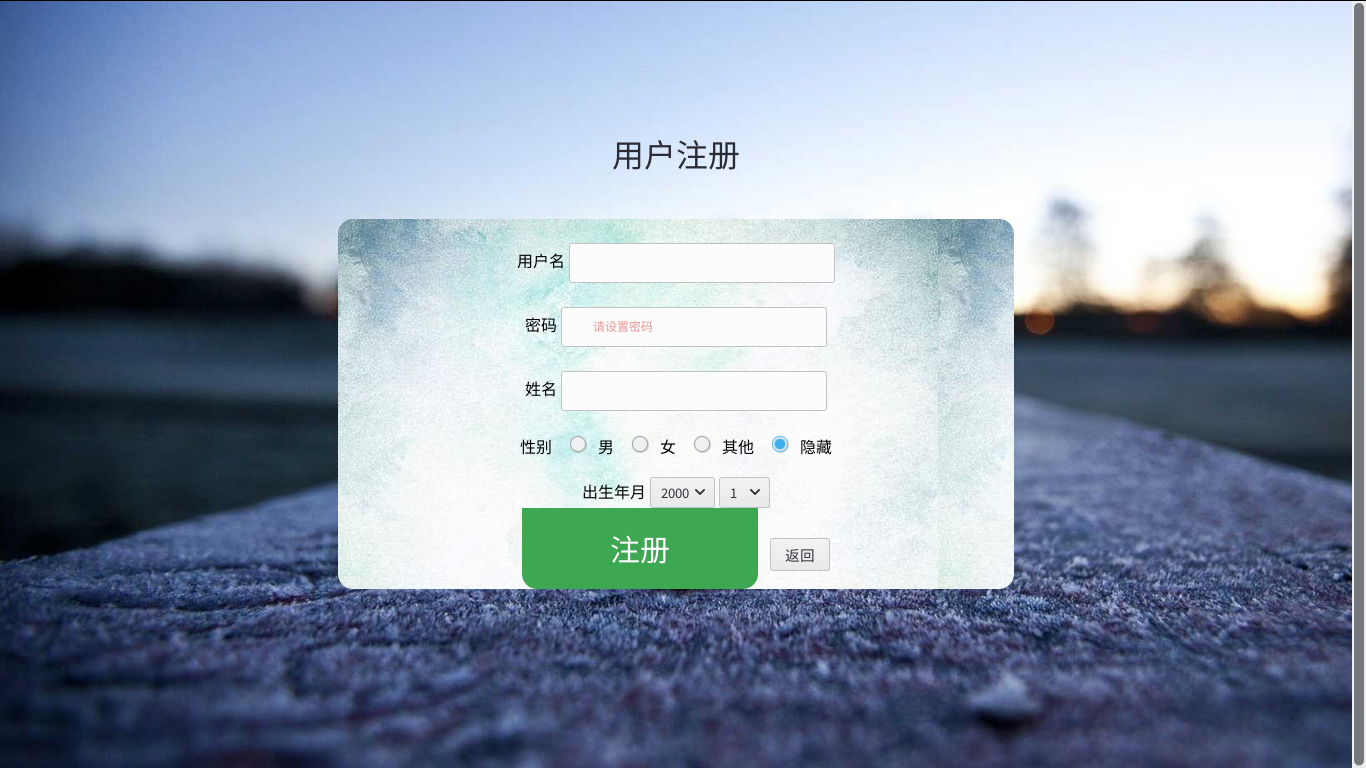
\includegraphics[scale=0.25]{register.png}
\end{center}

用户注册就是在 \mintinline{text}{account} 表中增加一条记录. 在增加记录之前首先检查用户名是否有重复.
\begin{minted}{sql}
SELECT * FROM `account` WHERE user_id = |\ttvariable{user\_id}| LIMIT 1;
\end{minted}
然后再插入新用户的记录.
\begin{minted}{sql}
INSERT INTO
`account` (user_id, password, user_name, sex, birth_year, birth_month)
VALUES (|\ttvariable{user\_id}|, |\ttvariable{password}|, |\ttvariable{user\_name}|, |\ttvariable{sex}|, |\ttvariable{birth\_year}|, |\ttvariable{birth\_month}|);
\end{minted}

\begin{center}
	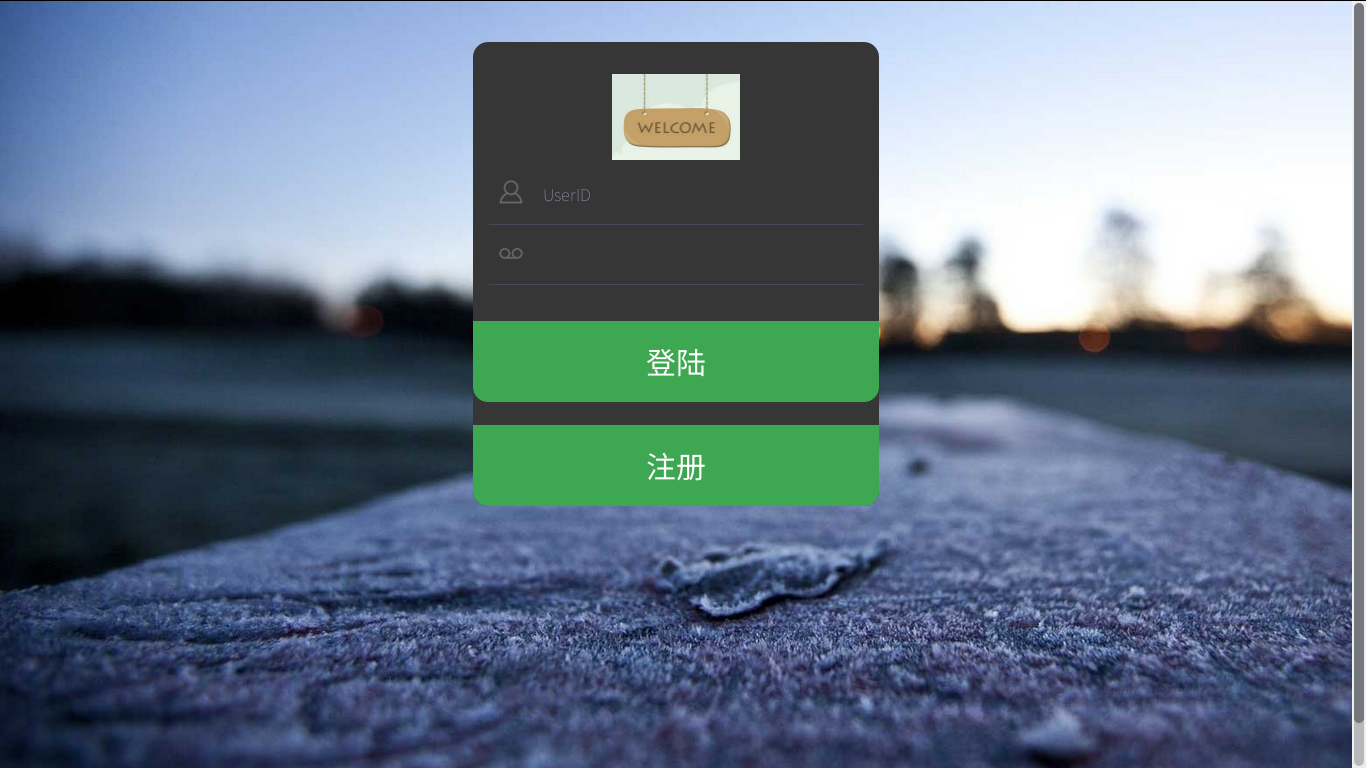
\includegraphics[scale=0.25]{login.png}
\end{center}

用户登录就是检查输入的用户名和密码是否与数据库中的记录匹配. 从数据库中查询该用户对应的密码.
\begin{minted}{sql}
SELECT password FROM `account` WHERE user_id = |\ttvariable{user\_id}| LIMIT 1;
\end{minted}
然后再检查是否和用户输入的密码匹配.

\subsection{关注好友和取消关注}

\begin{center}
	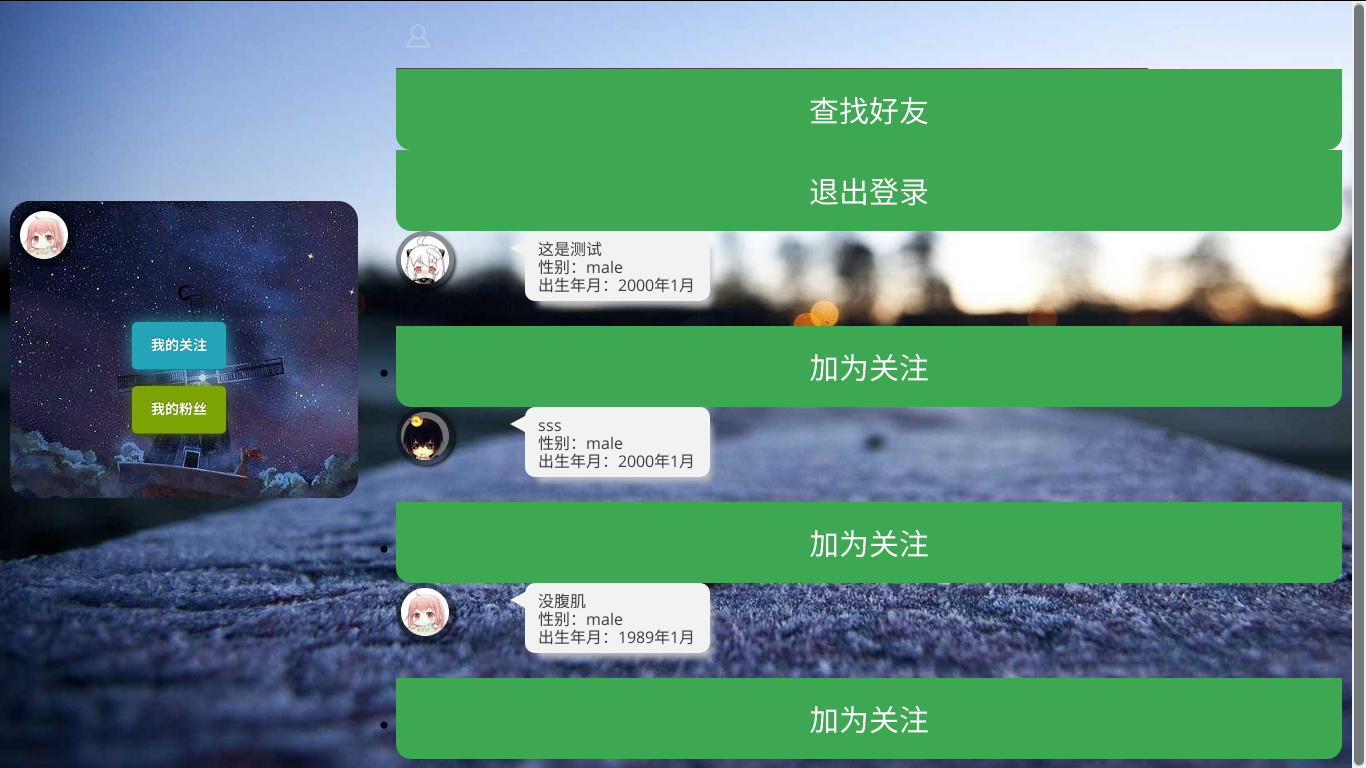
\includegraphics[scale=0.25]{search.png}
\end{center}

关注好友功能分为两步: 按名称搜索好友, 添加好友.

按名称搜索好友使用了数据库的模糊查找功能.
\begin{minted}{sql}
SELECT * FROM `account`
WHERE user_name like %|\ttvariable{search\_name}|%
AND user_id != |\ttvariable{user\_id}|  -- 排除自己
AND user_id NOT IN (  -- 排除已关注好友
    SELECT friend_id FROM `friends` WHERE user_id = |\ttvariable{user\_id}|);
\end{minted}

添加关注好友就是在 \mintinline{text}{friends} 表中添加一条记录.
\begin{minted}{sql}
INSERT INTO `friends` VALUES (|\ttvariable{user\_id}|, |\ttvariable{friend\_id}|);
\end{minted}

取消关注好友与之相反, 删除 \mintinline{text}{friends} 表中的相应记录.
\begin{minted}{sql}
DELETE FROM `friends`
WHERE user_id = |\ttvariable{user\_id}| AND friend_id = |\ttvariable{friend\_id}|;
\end{minted}

\subsection{发布、查看和回复状态}

发布状态就是在 \mintinline{text}{statement} 表中添加一条记录.
\begin{minted}{sql}
INSERT INTO `statement` (user_id, post_time, content)
VALUES (|\ttvariable{user\_id}|, |\ttvariable{post\_time}|, |\ttvariable{content}|);
\end{minted}

回复状态就是在 \mintinline{text}{comment} 表中添加一条记录.
\begin{minted}{sql}
INSERT INTO `comment` (user_id, statement_id, post_time, content)
VALUES (|\ttvariable{user\_id}|, |\ttvariable{statement\_id}|, |\ttvariable{post\_time}|, |\ttvariable{content}|);
\end{minted}

查看状态时, 要同时拉取状态和回复. 由于网页中回复显示在相应评论的下方, 我们需要分别查询每一条状态的回复, 而不是把它们一股脑地读出来.
\begin{minted}{sql}
SELECT a.user_id as user_id, user_name, avatar_index,
       statement_id, post_time, content
FROM `account` as a, `statement` as b
WHERE a.user_id = b.user_id AND b.user_id = |\ttvariable{friend\_id}|
ORDER BY post_time DESC LIMIT 10;
\end{minted}
\begin{minted}{sql}
SELECT a.user_id as user_id, user_name, avatar_index,
       comment_id, post_time, content
FROM `account` as a, `comment` as b
WHERE a.user_id = b.user_id AND b.statement_id = |\ttvariable{statement\_id}|
ORDER BY post_time;
\end{minted}

\subsection{主页自动更新状态}

\begin{center}
	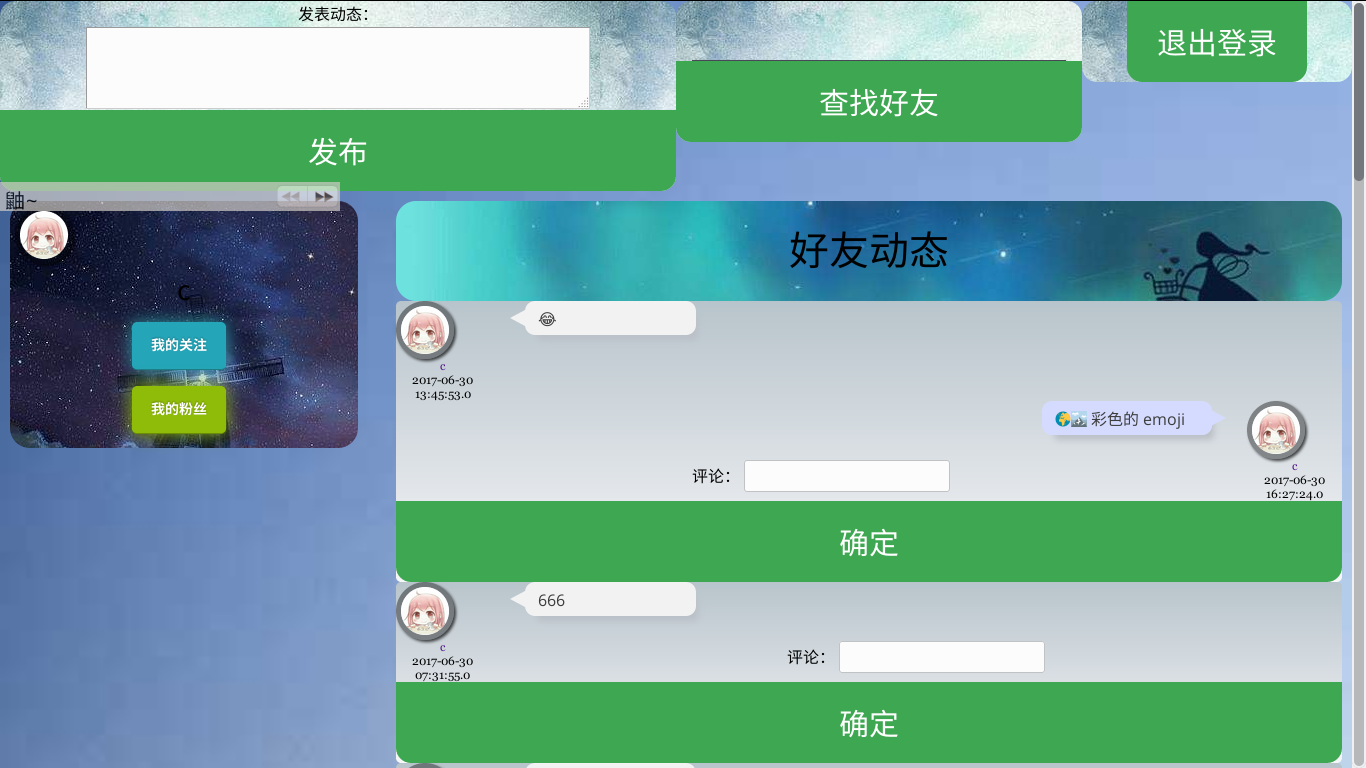
\includegraphics[scale=0.25]{homepage.png}
\end{center}

主页上不仅要显示自己的状态, 还要显示关注的好友的状态.
\begin{minted}{sql}
SELECT a.user_id as user_id, user_name, avatar_index,
statement_id, post_time, content
FROM `account` as a, `statement` as b
WHERE a.user_id = b.user_id
AND (b.user_id = |\ttvariable{user\_id}|
    OR b.user_id IN (
        SELECT friend_id FROM `friends` WHERE user_id = |\ttvariable{user\_id}|))
ORDER BY post_time DESC LIMIT 10;
\end{minted}

主页状态的自动更新通过 JavaScript 定时器实现.
\begin{minted}{javascript}
function myrefresh() {
    window.location.reload();
}
setTimeout('myrefresh()', 30000); // 指定 30 秒刷新一次
\end{minted}

\subsection{好友的好友信息}

查询好友中有多少好友也在关注.
\begin{minted}{sql}
SELECT * FROM `account`
WHERE user_id IN (
    SELECT a.friend_id FROM `friends` as a,`friends` as b
    WHERE a.user_id = |\ttvariable{user\_id}|
    AND b.friend_id = |\ttvariable{friend\_id}|
    AND a.friend_id = b.user_id);
\end{minted}

\section{部署环境}

本程序部署在一台 Linux 虚拟机上. 该虚拟机的硬件配置如下.
\begin{center}
	\begin{tabular}{c|c} \hline
		CPU & Intel Xeon X5 @ 2.4 GHz, 1 core \\ \hline 
		内存 & 1 GiB \\ \hline
		硬盘 & 20 GiB \\ \hline
		网络 & 1 Gbps \\ \hline
	\end{tabular}
\end{center}

服务器上的软件版本如下.
\begin{center}
	\begin{tabular}{c|c} \hline
		发行版 & Arch Linux \\ \hline 
		内核 & 4.11.6 \\ \hline
		nginx & 1.13.1 \\ \hline
		OpenJDK & 8u131 \\ \hline
		Tomcat & 8.0.44 \\ \hline
		MariaDB & 10.1.24 \\ \hline
		MySQL Connector/J & 5.1.41 \\ \hline
	\end{tabular}
\end{center}

本程序的部署采用了 Web 服务器和应用服务器分离的策略. Nginx 作为 Web 服务器, 工作在反向代理模式, 将客户端的 HTTPS 请求做 SSL 卸载, 把 HTTP 请求转发给 Tomcat 应用服务器. Tomcat 作为应用服务器, 专门处理 JSP 和 Servlet 部分.

\section{其他特性}

\subsection{用 Git 管理开发流程}

在本程序的开发过程中, 我们使用 Git 进行版本管理. Git 为开发过程带来了许多好处:
\begin{itemize}
	\item 完善的协作开发功能, 可以很好地处理开发过程中的文件冲突;
	\item 完整的历史版本记录, 程序出问题时可以方便地切换回旧版本;
	\item 利用 Git hook 功能, 我们实现了代码提交之后的自动部署, 保证服务器上随时运行最新版本的程序, 方便开发调试.
\end{itemize}

\subsection{Emoji 表情支持}

我们的程序支持 emoji 表情! 虽然不支持上传图片功能, 但 emoji 表情同样能带来令人惊艳的表现能力.

\begin{center}
	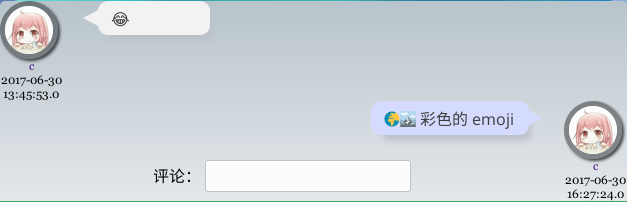
\includegraphics[scale=0.6]{emoji.png}
\end{center}

在 MySQL 和 MariaDB 中, 支持 emoji 表情的关键是所有程序都要使用支持 Unicode 扩展平面的编码. MySQL 和 MariaDB 默认使用的编码被称作 ``utf8'', 但它并不等同于标准的 UTF-8 编码, 它只支持 1 到 3 字节的 UTF-8 字符. 要使用 emoji 表情, 必须把 MySQL 和 MariaDB 的编码设置为 ``utf8mb4'', 以支持 4 字节的 UTF-8 字符 (大多数 emoji 表情都被编码为 4 字节 UTF-8 字符).

\subsection{HTTPS 和 HTTP/2 支持}

分离的 Web 服务器和应用服务器为我们带来了许多新的可能性, 其中之一就是对 HTTP 协议提供更完整的支持.

\begin{center}
	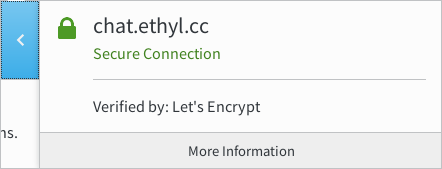
\includegraphics[scale=0.6]{https.png}
\end{center}

HTTPS 提供了卓越的安全性, 并且为我们减少了很多额外的工作.\footnote{当然, Tomcat 的默认 Web 服务器也支持 HTTPS, 但 nginx 的配置更加灵活, 并且加密/解密性能更优.} 例如, 由于 HTTPS 本身就使用加密传输, 我们的网页和服务器交互的信息就不用再考虑加密的问题了.

HTTP/2 协议优化了高延迟网络下的访问速度. Tomcat 8 的默认 Web 服务器并不支持这一功能. 我们的测试结果表明, 通过 nginx 反向代理开启 HTTP/2 支持之后, 页面加载时间比直接用 Tomcat 8 的默认 Web 服务器减少了 $40\%$ 左右.

\subsection{IPv6 网络支持}

\begin{center}
	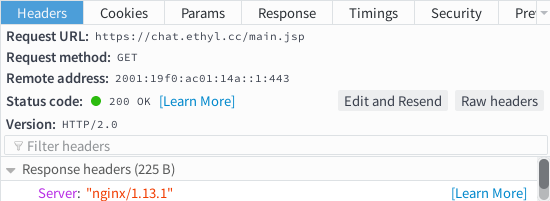
\includegraphics[scale=0.6]{h2+ipv6.png}
\end{center}

我们的服务器对 IPv4 和 IPv6 访问提供了同等的支持. 通过启用 IPv6 支持, 我们的程序能够运行在更多的网络环境下, 并且对校园网用户提供免费高速的优质体验.

\section{分工情况}

\paragraph{伏贵荣}
完成了以下功能:
\begin{itemize}
	\item 注册和登录界面;
	\item ``我的粉丝'' 和 ``我的关注''.
\end{itemize}

\paragraph{郭一江}
完成了以下功能:
\begin{itemize}
	\item 头像;
	\item 主页和状态;
	\item 好友搜索.
\end{itemize}

\paragraph{曾浩}
完成了以下功能:
\begin{itemize}
	\item 部署服务器环境;
	\item 程序访问数据库模块;
	\item 修复了一些 bug;
	\item 撰写文档.
\end{itemize}

程序代码中, 更具体的工作参见 Git 提交记录.

\end{document}